\section{Generating implicit ratings}

As discussed in Section~\ref{implicit-feedback} we can generate ratings based
on observed user behaviours in order to create a better experience for the
users, by not asking them to explicitly rate items, and we utilize valuable
information often found in access-logs and so forth. Hence, by having robust
methods for generating (implicit) ratings based on these logs we can create
common recommender systems models and recommend items without the user actively
taking part of the process.

\subsection{Levels of frequency, with global popularity}

Considering the weaknesses presented in Section~\ref{levels-frequency}, namely
choosing good weights and only using a small percentage of the scale between
0-100. Further, the method presented does not differentiate between active and
less active users, thus ignoring the entropy once the maximal level is reached.
Instead we extend the method by considering the global popularity of each item,
so that the user that.. % \todo{Finish the subsection about improving leveled
freq}

\subsection{Introduction to the sigmoid-function}

Extending our models further we want to capture our intuition that recent
events should count more towards a good rating, compared to old events. We
differentiate between two ways of classifying an event $e_u$ as old or recent;
one where we count the number of days between the newest event $e_n$ and event
$e_u$; and the second where we count the number of other events between $e_n$
and $e_u$. However, intuitively we consider a user to have multiple relevant
items concurrently and we know that in domains such as technology, fashion and
other consumer-products an item has an ago of relevancy, somewhat metaphoric to
a seasonal threshold. An example of this could be a fashion store recommending
warm clothes in the months between December to March, but then want to "change"
product pool based on the users behaviours – who are probably looking for
lighter clothes (changing season).

By considering recentness we also implicitly add negative feedback to events,
as in practice we are penalizing the ratings for old events. This is an
important aspect to keep in mind when working with implicit feedback, as
discussed in Section~\ref{implicit-feedback} as modern recommender engines work
better when we are assuming ratings are based on both positive and negative
feedback.

In order to catch our intuition mathematically we use a logistic function, which
is a mathematical function having an "S" shape and a common special case of the
more general sigmoid-function. In its most simplest case the logistic function
is defined as:

\begin{figure}[h!]
  \center
  \begin{tabular}{m{5cm}c}
    \toprule
    \begin{equation*}
      f(x) = \frac{1}{1+\exp^{-x}}
    \end{equation*}
  &
    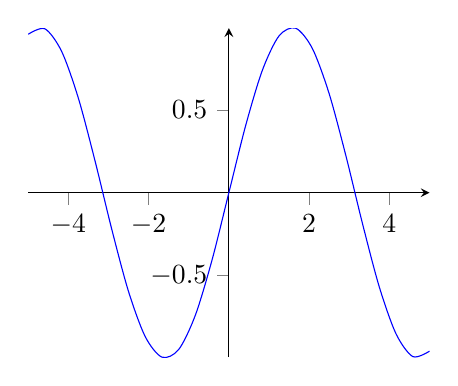
\begin{tikzpicture}
      \begin{axis}[width=190pt,axis x line=middle, axis y line=center, tick align=outside]
        \addplot+[mark=none,smooth] (\x,{sin(\x r)});
      \end{axis}
    \end{tikzpicture}
  \end{tabular}
\end{figure}

\subsection{Considering number of days since event}

\subsection{Considering ordering of events}

\subsection{Linearly blending the results}
